\documentclass[tikz,border=12pt]{standalone}
\usepackage[T1]{fontenc}
\usepackage{tgheros}
\usepackage{sfmath}
\usepackage{amsmath}
\usepackage{amssymb}
% % \usepackage{fontawesome5} (Removed for publication-grade academic typography) (Removed for publication-grade academic typography)
\usepackage{tikz}
\usetikzlibrary{arrows.meta,positioning,shapes.geometric,fit,backgrounds,calc}
\usepackage{xcolor}

\renewcommand{\familydefault}{\sfdefault}

% Academic Semantic Palette
\definecolor{harvardcrimson}{HTML}{A51C30}
\definecolor{ethdarkblue}{HTML}{1F407A}
\definecolor{ethblue}{HTML}{215CAF}
\definecolor{ethpetrol}{HTML}{007A87}
\definecolor{ethbronze}{HTML}{B87333}
\definecolor{ethpurple}{HTML}{5B4B8A}
\definecolor{ethslate}{HTML}{475569}
\definecolor{cardbg}{HTML}{F8FAFC}
\definecolor{cardborder}{HTML}{CBD5E1}
\definecolor{safeTeal}{HTML}{10B981}
\definecolor{proposalAmber}{HTML}{C98218}

\begin{document}
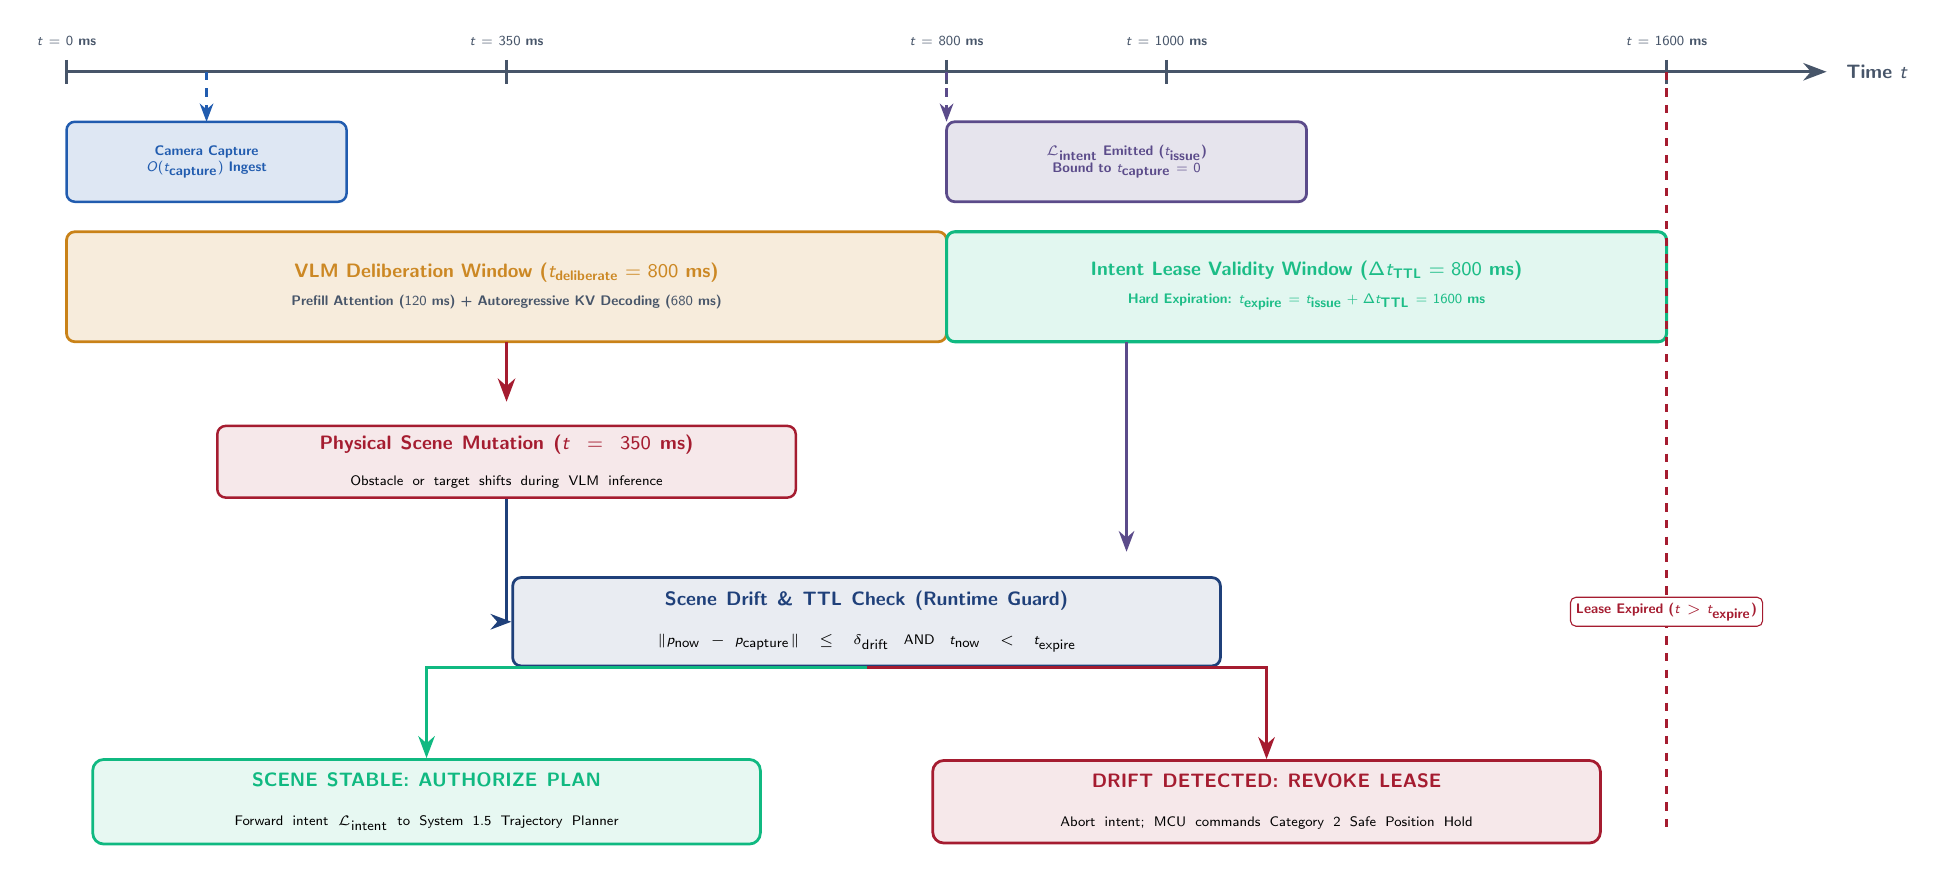
\begin{tikzpicture}[
  font=\sffamily,
  >=Stealth
]

  % Time Axis
  \draw[->, line width=1.2pt, draw=ethslate] (0, 0) -- (8.80in, 0);
  \node[anchor=west, font=\scriptsize\bfseries, text=ethslate] at (8.85in, 0) {Time $t$};

  % Time Tick Marks
  \foreach \x/\lbl in {0/{$t=0\text{ ms}$}, 2.20/{$t=350\text{ ms}$}, 4.40/{$t=800\text{ ms}$}, 5.50/{$t=1000\text{ ms}$}, 8.00/{$t=1600\text{ ms}$}} {
    \draw[line width=0.8pt, draw=ethslate] (\x in, 0.06in) -- (\x in, -0.06in);
    \node[font=\tiny\bfseries, text=ethslate, anchor=south] at (\x in, 0.08in) {\lbl};
  }

  % Row 1: Instantaneous Events
  % Camera Ingest
  \draw[fill=ethblue!15, draw=ethblue, line width=0.9pt, rounded corners=3pt] (0, -0.65in) rectangle ++(1.40in, 0.40in);
  \node[font=\tiny\bfseries, text=ethblue, align=center] at (0.70in, -0.45in) {Camera Capture\\$O(t_{\text{capture}})$ Ingest};
  \draw[->, line width=0.8pt, draw=ethblue, dashed] (0.70in, 0) -- (0.70in, -0.25in);

  % Intent Lease Emitted
  \draw[fill=ethpurple!15, draw=ethpurple, line width=1pt, rounded corners=3pt] (4.40in, -0.65in) rectangle ++(1.80in, 0.40in);
  \node[font=\tiny\bfseries, text=ethpurple, align=center] at (5.30in, -0.45in) {$\mathcal{L}_{\text{intent}}$ Emitted ($t_{\text{issue}}$)\\Bound to $t_{\text{capture}} = 0$};
  \draw[->, line width=0.8pt, draw=ethpurple, dashed] (4.40in, 0) -- (4.40in, -0.25in);

  % Row 2: Intervals / Windows
  % Deliberation Block
  \draw[fill=proposalAmber!15, draw=proposalAmber, line width=1pt, rounded corners=3pt] (0, -1.35in) rectangle (4.40in, -0.80in);
  \node[font=\scriptsize\bfseries, text=proposalAmber!95, align=center] at (2.20in, -1.07in) {
    VLM Deliberation Window ($t_{\text{deliberate}} = 800\text{ ms}$)\\[2pt]
    {\tiny\color{ethslate}Prefill Attention ($120\text{ ms}$) + Autoregressive KV Decoding ($680\text{ ms}$)}
  };

  % Lease TTL Valid Window
  \draw[fill=safeTeal!12, draw=safeTeal, line width=1.1pt, rounded corners=3pt] (4.40in, -1.35in) rectangle (8.00in, -0.80in);
  \node[font=\scriptsize\bfseries, text=safeTeal!95, align=center] at (6.20in, -1.07in) {
    Intent Lease Validity Window ($\Delta t_{\text{TTL}} = 800\text{ ms}$)\\[2pt]
    {\tiny Hard Expiration: $t_{\text{expire}} = t_{\text{issue}} + \Delta t_{\text{TTL}} = 1600\text{ ms}$}
  };

  % Hard Expiration Vertical Line
  \draw[dashed, line width=1.2pt, draw=harvardcrimson] (8.00in, 0) -- (8.00in, -3.80in);
  \node[font=\tiny\bfseries, fill=white, draw=harvardcrimson, rounded corners=2pt, inner sep=2pt, text=harvardcrimson] at (8.00in, -2.70in) {Lease Expired ($t > t_{\text{expire}}$)};

  % Row 3: Physical Scene Mutation Event
  \draw[->, line width=1.2pt, draw=harvardcrimson] (2.20in, -1.35in) -- (2.20in, -1.65in);
  \node[draw=harvardcrimson, fill=harvardcrimson!10, rounded corners=3pt, line width=0.9pt, text width=2.80in, align=center] (mutation) at (2.20in, -1.95in) {
    {\scriptsize\bfseries\color{harvardcrimson} Physical Scene Mutation ($t = 350\text{ ms}$)}\\[1pt]
    {\tiny Obstacle or target shifts during VLM inference}
  };

  % Row 4: Decision Check
  \node[draw=ethdarkblue, fill=ethdarkblue!10, rounded corners=3pt, line width=1.0pt, text width=3.40in, inner sep=5pt, align=center] (check) at (4.00in, -2.75in) {
    {\scriptsize\bfseries\color{ethdarkblue} Scene Drift \& TTL Check (Runtime Guard)}\\[2pt]
    {\tiny $\|p_{\text{now}} - p_{\text{capture}}\| \le \delta_{\text{drift}} \quad \text{AND} \quad t_{\text{now}} < t_{\text{expire}}$}
  };

  \draw[->, line width=1pt, draw=ethdarkblue] (mutation.south) |- (check.west);
  \draw[->, line width=1pt, draw=ethpurple] (5.30in, -1.35in) -- (5.30in, -2.40in);

  % Row 5: Branches
  \node[draw=safeTeal, fill=safeTeal!10, rounded corners=4pt, line width=1pt, text width=3.20in, inner sep=5pt, align=center] (nominal) at (1.80in, -3.65in) {
    {\scriptsize\bfseries\color{safeTeal} SCENE STABLE: AUTHORIZE PLAN}\\[2pt]
    {\tiny Forward intent $\mathcal{L}_{\text{intent}}$ to System 1.5 Trajectory Planner}
  };

  \node[draw=harvardcrimson, fill=harvardcrimson!10, rounded corners=4pt, line width=1pt, text width=3.20in, inner sep=5pt, align=center] (veto) at (6.00in, -3.65in) {
    {\scriptsize\bfseries\color{harvardcrimson} DRIFT DETECTED: REVOKE LEASE}\\[2pt]
    {\tiny Abort intent; MCU commands Category 2 Safe Position Hold}
  };

  \draw[->, line width=1.1pt, draw=safeTeal] (check.south) -| (nominal.north);
  \draw[->, line width=1.1pt, draw=harvardcrimson] (check.south) -| (veto.north);

\end{tikzpicture}
\end{document}
